\chapter{Stima della distanza con RSSI, Android e tecnologie BLE}

\section{Sviluppare un'app Android compatibile con BLE}
L'obiettivo dell'app è far interagire un cellulare (con sistema operativo Android) con gli iBeacon disposti in una stanza. Dalle API 18 in poi Android integra nativamente la comunicazione e ricezione dati su protocollo Bluetooth LE.

Visto che l'applicazione non funziona senza questa specifica, nell'\texttt{AndroidManifest.xml} sono state imposte delle condizioni che inibiscono l'installazione dell'app a dispositivi che non hanno una radio Bluetooth Low Energy.

\begin{lstlisting}[language=XML]
<uses-permission android:name="android.permission.BLUETOOTH" />
<uses-permission android:name="android.permission.BLUETOOTH_ADMIN" />
<uses-feature android:name="android.hardware.bluetooth_le" android:required="true" />
\end{lstlisting}

Al fine di inibire l'installazione a smartphone con API minori a 18, nel file \texttt{build.gradle} è stata inserita la regola:
\begin{lstlisting}[language=Java]
    defaultConfig {
    	...
    	minSdkVersion 18
    	...
    }
\end{lstlisting}

\section{Compatibilità con Android 5.0+}
Per rendere eseguibile l'app a smarphone con Android dalla versione 5.0 in poi è stato aggiunto un metodo (\texttt{checkAndroidMPermission()}) per fare il check dei permessi di Android. Senza questo accorgimento l'app sarebbe stata installata ma non avrebbe funzionato la scansione dei dispositivi BT.

\subsubsection{Controllo della compatibilità con Android 5.0+}
\begin{lstlisting}[language=Java]
private void checkAndroidMPermission() {
   	
   	if (Build.VERSION.SDK_INT >= Build.VERSION_CODES.M) {
   		final List<String> permissions = new ArrayList<>();
   		
   		if (checkSelfPermission(Manifest.permission
		   	.ACCESS_FINE_LOCATION)
		   		!= PackageManager.PERMISSION_GRANTED) {
   			permissions.add(Manifest.permission
	   			.ACCESS_FINE_LOCATION);
   		}
   		
   		if (checkSelfPermission(Manifest.permission
	   		.ACCESS_COARSE_LOCATION)
		   		!= PackageManager.PERMISSION_GRANTED) {
   			permissions.add(Manifest.permission
	   			.ACCESS_COARSE_LOCATION);
   		}
   		
   		if (!permissions.isEmpty()) {
   			new AlertDialog.Builder(this)
   			.setTitle(R.string.dialog_location_access_title)
   			.setMessage(R.string.dialog_bluetooth_text)
   			.setPositiveButton(android.R.string.ok, null)
   			.setOnDismissListener(new DialogInterface.OnDismissListener() {
   				@TargetApi(23)
   				@Override
   				public void onDismiss(DialogInterface dialog) {
   					requestPermissions(permissions.toArray(
	   					new String[permissions.size()]),
   					REQUEST_CODE_ASK_MULTIPLE_PERMISSIONS);
   				}
   				
   			}).show();
   		}
   	}
}
\end{lstlisting}

\section{Libreria AltBeacon - android-beacon-library}
Per estendere il supporto nativo fornito alla connettività Bluetooth è stata utilizzata la libreria \href{https://github.com/AltBeacon/android-beacon-library}{\textbf{AltBeacon}}\footnote{\href{https://github.com/AltBeacon/android-beacon-library}{\textbf{AltBeacon}} - \url{https://github.com/AltBeacon/android-beacon-library}}. Questa permette di generare delle regioni di interesse, degli avvisi all'utente, filtrare i dispositivi BT, ecc. Con essa è inoltre fornito un modulo per il risparmio energetico.

Per l'inclusione di questa libreria si inserita la seguente stringa nel file \texttt{build.gradle}.
\begin{lstlisting}[language=Java]
dependencies {
	...
	// android beacon library AltBeacon
	compile 'org.altbeacon:android-beacon-library:2.9.1'
	...
}
\end{lstlisting}

\section{Calcolo della distanza RAW}
La stima della distanza in base ai RSSI calcolati si esegue nel metodo \texttt{calculateDistance(double txPower, double rssi)}.

\subsubsection{Stima della distanza in base agli RSSI}
\begin{lstlisting}[language=Java]
// radiousNetwork formula
private double calculateDistance(double txPower, double rssi) {
	
	if (rssi == 0.0D) {
		return -1.0D; // if we cannot determine accuracy, return -1.
	}
	
	double ratio = (rssi * 1.0D) / txPower;
	if (ratio < 1.0D) {
		return Math.pow(ratio, 10.0D);
	}
	
	return (0.89976D * Math.pow(ratio, 7.7095D)) + 0.111D;
}
\end{lstlisting}

\section{Filtri}
Per ridurre le problematiche di rilevamento di RSSI(\ref{ch:problematiche}) sono stati sviluppati e/o utilizzati tre filtri: RunningAverageRssi, filtro di Kalman, filtro ARMA. Questi possono essere combinati tra loro senza inficiare le prestazioni del sistema. Presentano delle parametrizzazioni controllabili dal \textit{Settings} per adattarsi a tutti vari contesti di stima.

Per scelta progettuale il filtro di Kalman è sempre attivo. Si è fatto in modo che il valore filtrato col questo filtro sia confrontabile con la misurazione della distanza RAW e con quella filtrata dalla libreria AltBeacon.

\subsection{Filtro RunningAverageRssi}
Il filtro \textit{RunningAverageRssi} calcola il valore RSSI sulla base di un elenco arbitrario di valori RSSI misurati. L'elenco viene troncato da una certa lunghezza all'inizio e alla fine. Il valore calcolato è una semplice media aritmetica. Viene fornito dalla libreria AltBeacon come filtro di default, ma non sembra essere particolarmente preciso.

\subsection{Implementazione del filtro di Kalman}

Per realizzare il filtro di Kalman sono state utilizzate tre classi: 
\begin{itemize}
	\item \texttt{KFilterBuilder}: per creare un filtro di Kalman unidimensionale;
	\item \texttt{KFilter}: per il filtraggio vero e proprio.
	\item \texttt{Estimation}: per implementare il filtro sui valori di input.
\end{itemize}
Parametri passati a KFilter:
\begin{itemize}
	\item R = rumore di processo;
	\item Q = misurazione del rumore;
	\item A = vettore di stato;
	\item B = vettore di controllo;
	\item C = vettore delle misurazioni.
\end{itemize}

Questo filtro è inizializzato nella classe \texttt{Estimation} (istanziata volta alla creazione di degli oggetti \textit{Device}). Ogni volta che viene richiamato il metodo \texttt{updateDistance(Beacon b, double processNoise)} di \texttt{EStimation};
\begin{itemize}
	\item si aggiunge un nuovo valore alla variabile \texttt{recentRSSI}, istanza di un oggetto \texttt{DescriptiveStatistics}
	\item si aggiunge un nuovo valore alla variabile \texttt{recentTxPower}, istanza di un oggetto \texttt{DescriptiveStatistics}
	\item si calcola il nuovo valore di rumore in base ai nuovi input
	\item se il nuovo valore di rumore non è un numero infinito e non è un Not-a-Number, si passa al metodo \texttt{setMeasurementNoise(mNoise)} di \texttt{KFilter}
	\item si setta il nuovo rumore di processo, che dipende dall'input dato da \texttt{Settings}
	\item si calcola la distanza con i parametri appena calcolati
\end{itemize}

\subsubsection{Filtraggio in base agli input}
\begin{lstlisting}[language=Java]
public void updateDistance(Beacon b, double processNoise) {
   	
   	recentRSSI.addValue(b.getRssi());
   	recentTxPower.addValue(b.getTxPower());
   	
   	// Update measurement noise continually
   	double mNoise = Math.sqrt((100 * 9 / Math.log(10)) *
   	Math.log(1 + Math.pow(recentRSSI.getMean() / recentRSSI.getStandardDeviation(), 2)));
   	
   	if (!Double.isInfinite(mNoise) && !Double.isNaN(mNoise)) {
   		kf.setMeasurementNoise(mNoise);
   	}
   	
   	kf.setProcessNoise(processNoise);
   	double lastFilteredReading = kf.filter(recentRSSI.getPercentile(50));
   	distanceEstimated = calculateDistance(recentTxPower.getPercentile(50), lastFilteredReading);
   	rawDistanceEstimated = calculateDistance(b.getTxPower(), b.getRssi());
   	WOSC = calculateDistance(b.getTxPower(), lastFilteredReading);
}
\end{lstlisting}

\subsubsection{Filtering nella classe KFilter}\label{ch:kfilter}
\begin{lstlisting}[language=Java]
/**
* Filter a new value
*
* @param z Measurement
* @param u Control
* @return x
*/
public double filter(double z, double u) {
   	
   	if (Double.isNaN(x)) {
   		x = (1 / C) * z;
   		x1 = x;
   		x2 = x1;
   		cov = (1 / C) * Q * (1 / C);
   	} else {
   	
    	// Calculate previous update step
    	B = (x - x1) / 2;
   	
    	// Compute prediction
    	double predX = (A * x) + (B * u);
    	double predCov = ((A * cov) * A) + R;
   	
    	// Kalman gain
    	double K = predCov * C * (1 / ((C * predCov * C) + Q));
    	
    	// Correction
    	x1 = x;
    	x = predX + K * (z - (C * predX));
    	cov = predCov - (K * C * predCov);
	}

	return x;
}
\end{lstlisting}

\subsection{Implementazione del filtro ARMA}\label{ch:filtro_arma}
Il filtro \textbf{ARMA} (\textit{Auto Regressive Moving Average}) calcola gli RSSI in base al valore corrente. Questo filtro è tradotto in codice nella classe \texttt{MyArmaRssiFilter} che implementa la classe \texttt{RssiFilter}.

Per il filtraggio degli RSSI si utilizza la formula\ref{eq:arma}:
\begin{equation}\label {eq:arma}
n(t) = n(t-1) - c (n(t-1) - n(t))
\end{equation} 
dove $ c $ è il coefficiente che denota l'uniformità (\textit{smoothness}). Più basso è questo valore più uniforme è la media.

Il metodo più importante di questa classe è \texttt{addMeasurement(Integer rssi)} dove si ricevono in input gli RSSI e si esegue il filtraggio in base al coefficiente $ c $ (qui tradotto nella variabile \texttt{armaSpeed}).

\subsubsection{Aggiornamento del filtro ARMA}
\begin{lstlisting}[language=Java]
@Override
public void addMeasurement(Integer rssi) {
    	
   	if (isEnabled) {
   		if (!isInitialized) {
   			armaMeasurement = rssi;
   			isInitialized = true;
   		}
   		armaMeasurement = (armaMeasurement - armaSpeed * (armaMeasurement - rssi));
   	} else {
    	armaMeasurement = rssi;
    }
}
\end{lstlisting}

Per il settaggio dinamico del coefficiente $ c $ si utilizza il metodo \texttt{setArmaSpeed(double arma\_speed)}. Visto che i segnali considerati tendono a variare piuttosto frequentemente (alla frequenza di 1Hz o superiore), il valore consigliato per 1HZ sarebbe 0,1 (cioè l'input viene modificato del 10\% della differenza tra la misurazione attuale e la media effettiva). Per segnali a frequenza superiori (10Hz) si consiglia un valore compreso tra 0,25 e 0,5.

\newpage
\subsection{Grafici in tempo reale}
Si è scelto di far visualizzare a schermo, direttamente dall'app, dei grafici in tempo reale in modo da rendere più chiaro l'andamento delle stime.
Per far questo è stata utilizzata la libreria \href{https://github.com/PhilJay/MPAndroidChart}{\textbf{MPAndroidChart}}\footnote{\href{https://github.com/PhilJay/MPAndroidChart}{\textbf{MPAndroidChart}} - \url{https://github.com/PhilJay/MPAndroidChart}}.

Per l'inclusione di questa libreria si inserita la seguente stringa nel file \texttt{build.gradle}.
\begin{lstlisting}[language=Java]
dependencies {
	...
	// chart library
	compile 'com.github.PhilJay:MPAndroidChart:v3.0.0-beta1'
	...
}
\end{lstlisting}

\subsubsection{Dettaglio di un grafico in tempo reale}
\begin{figure}[ph]
	\centering
	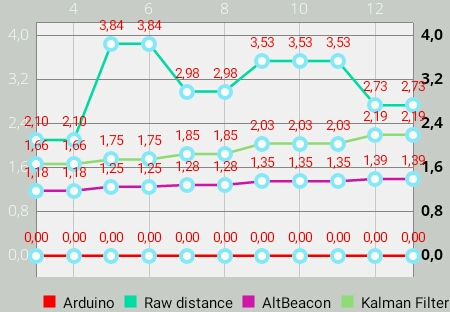
\includegraphics[width=0.6\linewidth]{img/app/chart1.jpg}
	\caption{Esempio di grafico in tempo reale}
	\label{fig:chart1}
\end{figure}



